\graphicspath{{chapters/02/images/}}
\chapter{Biocompatibility}

\section{Introduction}
Biocompatibility is an essential aspect to take into consideration for the specification of the medical device that is being designed.
Before building a scaffold or a biological device its time, location and individual in which it will be used need to be defined.
A scaffold to be useful should activate specific cellular function and reflect and exploit the different mechanical and chemical properties of the tissue in which it will be implanted.
Because of this, a scaffold should be designed taking into account the specific region in which it will be implanted, considering the cell population and kind of injury, as well as other parameters.
Cells are the building blocks of biology and they can read the information coming from the external environment.
Specific gene expression is activated in cells given external signalling molecules.
This makes it evident that the environment reaches the cell through chemical and mechanical stimuli.
Therefore, scaffolds are not self-sufficient entities: they are bioactive and need to collaborate with environment, cells and the extracellular matrix to perform their function.

	\subsection{Parameters defining biological outcome}
	The biological outcome that will be obtained depends on a list of parameters which, once defined, allow for the creation of a scaffold capable of regenerating the injured tissue.
	The parameters are:

	\begin{multicols}{2}
		\begin{description}
		\item[Porosity] is extremely important for cell migration.
			The material should be in 3D, as  the scaffold should allow and promote cell adhesion, growth and migration.
		\item[Mechanical properties] are different for each tissue, the scaffold should both resist physical stress and provide the correct stimulus that the cells need to grow, adhere, migrate and differentiate.
		\item[Surface] modification is often referred to the functionalization of the scaffold through the addition of proteins or sequences of amino acids to increase adherence.
		\item[Antibiotic/antiviral] drugs release system, to control chronic inflammation and possible infections.
		\item[Surface topography] may be smooth or rough for example.
		\end{description}
	\end{multicols}

	\subsection{Guided tissue regeneration - cartilage example}

		\begin{figure}[ht]
			\centering
			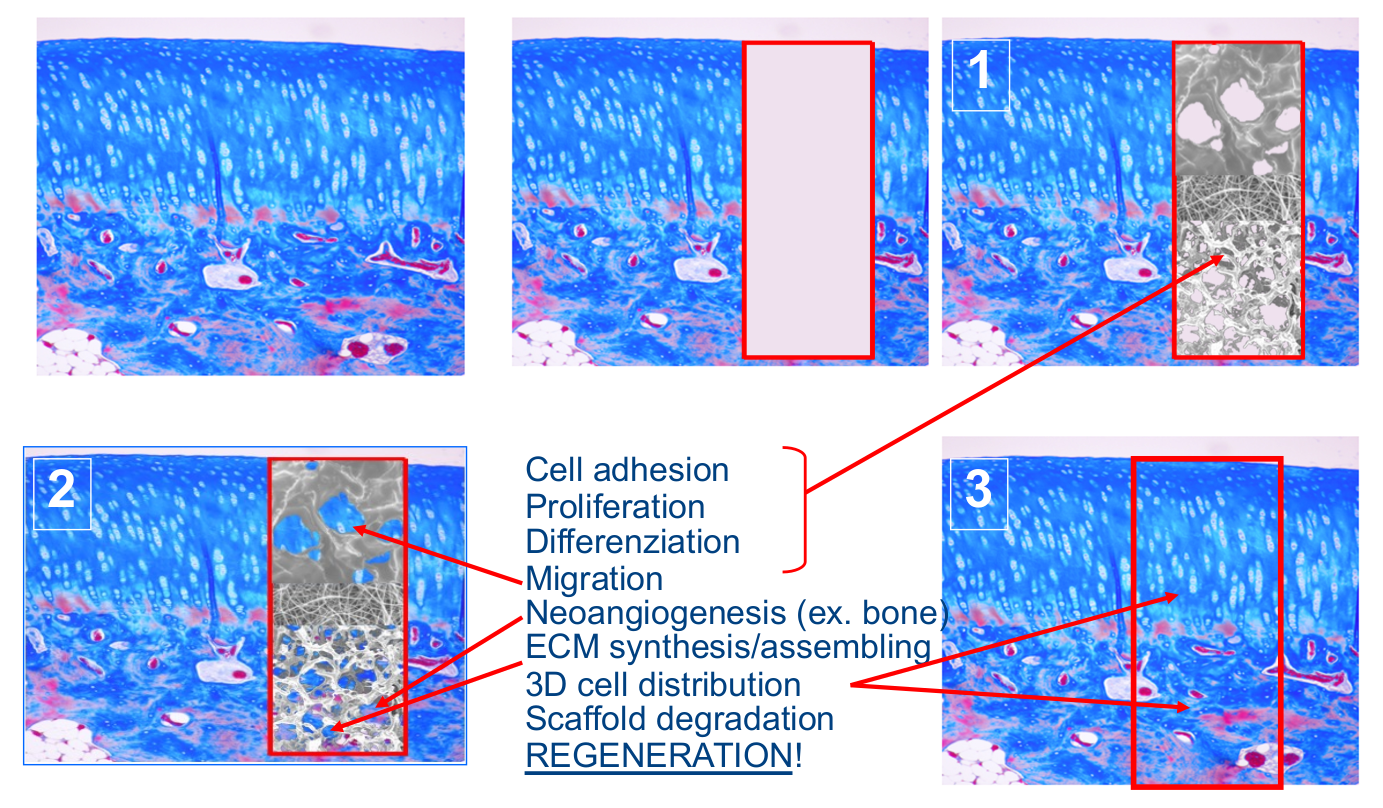
\includegraphics[width=0.5\textwidth]{cartilage.png}
			\caption{Cartilage regeneration}
			\label{fig:cartilage}
		\end{figure}

	In figure \ref{fig:cartilage} we can see an articular cartilage, an intermediate tissue and bone.
	These three different tissues present differences in vascularization, cell organization (in cartilage cells live in lacuna, where migration and proliferation are downregulated) and innervation.\\
	In case of trauma, most of the time the damage reaches the bone due to the lack of innervation in the cartilage.
	Because of this, a multi-component scaffold that accounts for different types of tissues is designed.
	In particular the scaffold should:

	\begin{multicols}{2}
		\begin{itemize}
			\item Upregulate angiogenesis in the bone and downregulate it in the cartilage.
			\item Increase the water content in cartilage, so as to increase its compressive capabilities through hydrophilic materials.
			\item Provide an environment for osteoblasts and lacunae for cartilage cells
			\item Provide space for nerves, vascularization and cell migration.
			\item Tissue specific degradation times.
		\end{itemize}
	\end{multicols}

	After the design, biocompatibility needs to be checked: it will have an impact on cell adhesion, proliferation, differentiation and migration, on neoangiogenesis and on the regeneration of the function of the damaged tissue.

	\subsection{The principles of tissue engineering}

	\begin{figure}[ht]
		\centering
		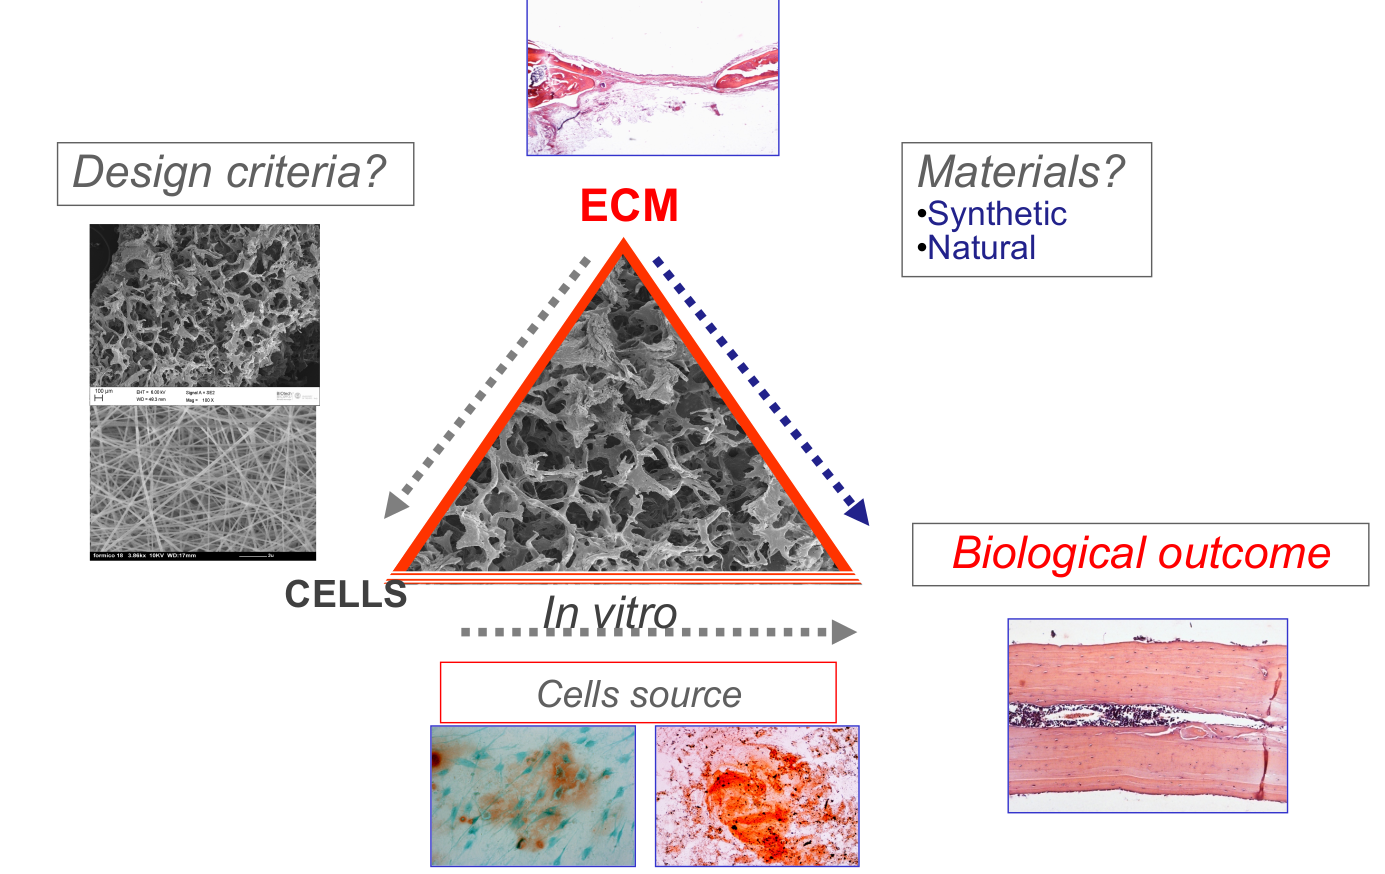
\includegraphics[width=0.5\textwidth]{triangolo.png}
		\caption{Tissue engineering principles}
		\label{fig:triangle}
	\end{figure}

	A tissue engineering process is composed by three steps:

	\begin{multicols}{3}
		\begin{itemize}
			\item Design.
			\item Material choice.
			\item In vitro and in vivo testing.
		\end{itemize}
	\end{multicols}

	Tissue engineering implements a multidisciplinary strategy and the advance in materials' science and biology drastically improve the success of scaffold application.
	The advances in biology, for example the discovery in $2000$ of macrophages \emph{M1} and \emph{M2}, allow for the design of more biocompatible scaffolds.


		\subsubsection{4th generation biological regenerative biomaterials}
		A biomaterial to be defined as a 4th generation biological regenerative biomaterial needs to:

		\begin{multicols}{2}
			\begin{itemize}
				\item Change its activity based on the environment: be, for example thermo or pH responsive.
				\item Be instructional: functionalized with peptides that can control cells' fate.
				\item Have specific mechanical strength and functions to allow for mechanical signalling.
			\end{itemize}
		\end{multicols}

	Biomaterials need to be stable and inert in the beginning to allow for drug delivery, for printing organ and for cell therapies.
	The hope for the future is to develop also diagnostic systems and to implant electronic devices.

\section{Definition}

	\subsection{First definition}
	At first a material was defined as biocompatible when inert, presenting a total absence of interaction between the material and the tissues.
	Minimal reaction to the foreign body was preferred, meaning no (or low) inflammatory reaction and no immuno-response.
	This definition focuses on the body reaction to the implant, requiring on the latter only chemical stability.

		\subsubsection{Problem with the first definition - heart valves}

		\begin{figure}[ht]
			\centering
			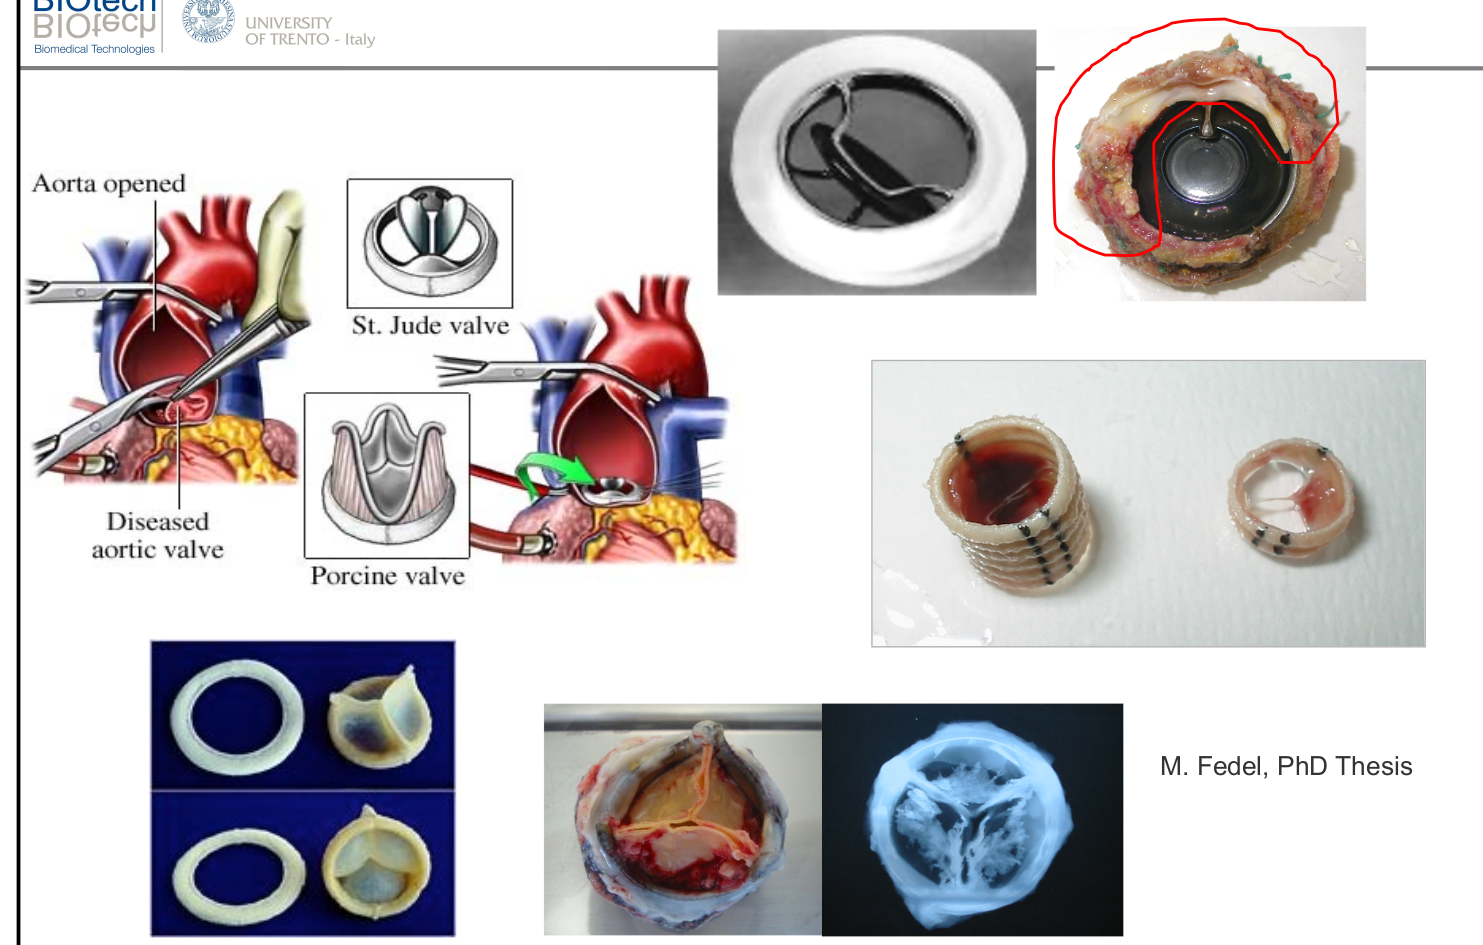
\includegraphics[width=0.5\textwidth]{valves.png}
			\caption{\label{fig:valves}}
		\end{figure}

		The issues with this definition were brought to light when observing the implant some time after the implantation.
		We will now discuss as an example the problem with heart valves.
		A heart valve made of titanium and polyester failed to induce regeneration because the body built a very thick scar tissue around the plastic layer, not letting it open anymore.
		The same valve with an ultra thin silver layer used for antibiotic purposes caused thrombosis in other patients.
		To tackle this problem, this valve was treated with anticoagulants.
		A biological heart valve harvested from pigs failed because of calcification, which rendered the valve unable to close.

	\subsection{Second definition}
	All materials induce a biological reaction.
	No material is completely inert, because our antibodies can recognize anything that is not "self".
	The concept of biocompatibility was revised as \textit{"the ability of a material to perform a specific application causing an appropriate host response in a specific application"} (1987).
	It is clear how the context of implantation is fundamental: scaffolds should be tissue and organ dependent, resolving a defined situation by reacting with the tissue and activating the cellular functions to heal a specific environment, before being degraded.

		\subsubsection{FBRx - an example}

		\begin{figure}[ht]
			\centering
			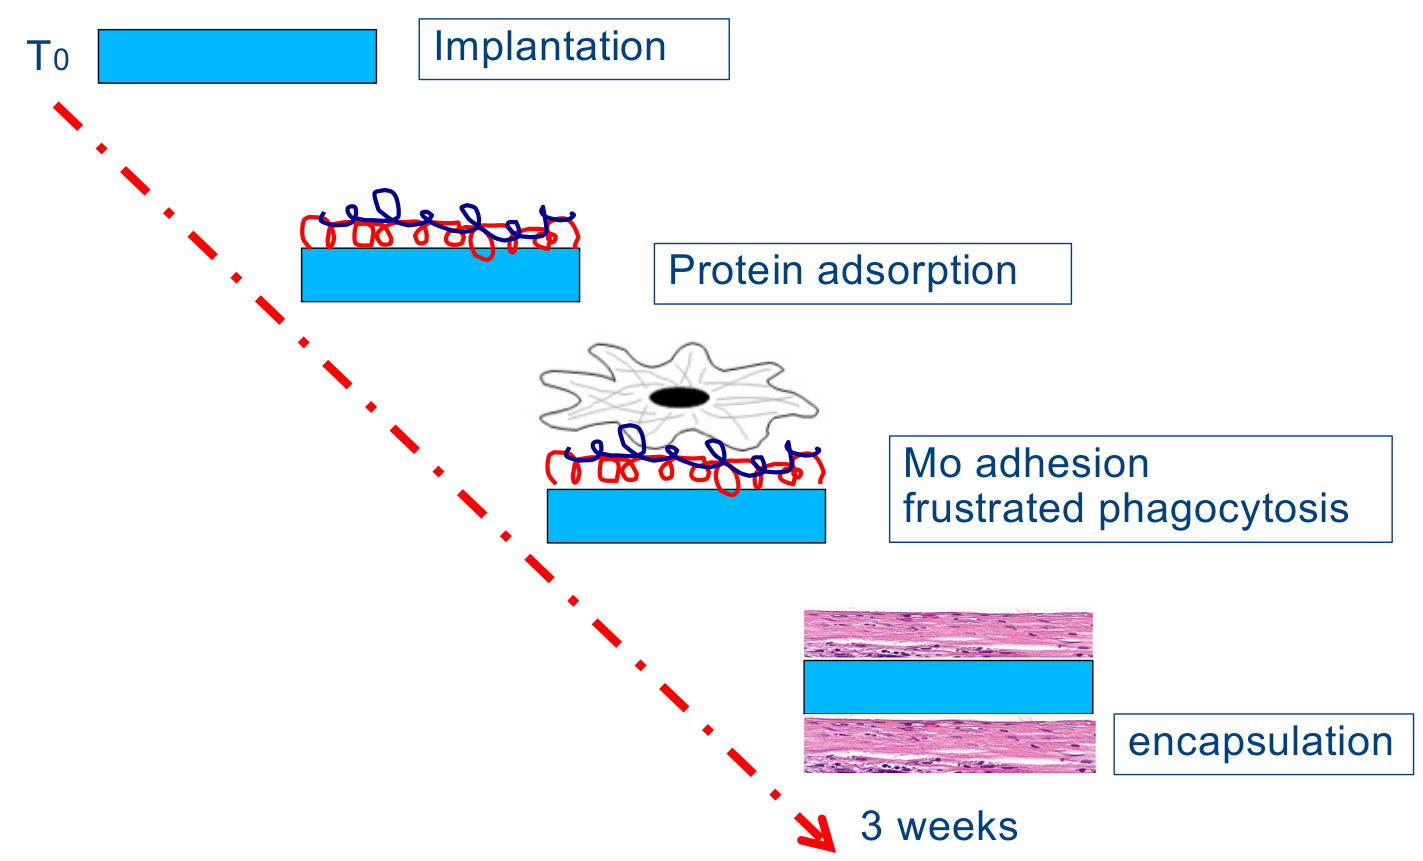
\includegraphics[width=0.5\textwidth]{fbrx.png}
			\caption{\label{fig:matrixome}}
		\end{figure}

		We can take as an example FBRx, a non porous scaffold material.
		Depending on the chemistry of the material, we can activate a specific protein adsorption and subsequently a specific immune response.
		If the material is not degradable, the macrophages start to coat the foreign body with scar tissue, ending the adsorption reaction, allowing the scaffold to degrade and leaving an empty bag of scar tissue.
		By changing the porosity, the scar tissue is reduced and regeneration is promoted.
		For this case injectable gels (hydrogels) are useful scaffolds: they are porous and leave space for cell migration.
		Because of this, they are used when filling cavities.

	\subsection{Re-evaluation of the biocompatibility concept}
	Some factors led to the redefinition of the concept of biocompatibility, as for the scaffold is not enough to simply exist.

	\begin{multicols}{2}
		\begin{itemize}
			\item Response to specific materials could vary from one application site to another, it is tissue-organ dependent: there is a need to define both material characteristics and implantation context, composed by the tissue and the injury.
			\item An increasing number of applications require that the material specifically reacts with the tissues, rather than being ignored by them.
			\item Some applications require that the material degrades over time in the body, rather than remaining indefinitely in it.
		\end{itemize}
	\end{multicols}

	Because of this, biocompatibility can be considered a system's property: it cannot be defined without considering the implantation context. It involves the separate, but interrelated, responses of the two phases of the biomaterial-tissue complex and interfacial phenomena triggered by their compact.
	The key to understand biocompatibility is:

	\begin{multicols}{2}
		\begin{itemize}
			\item The determination of which chemical, biochemical, physiological, physical or other mechanism become operative and why.
			\item The determination of the highly specific conditions associated with contact between biomaterials and tissue of the body.
			\item What are the consequences of these interactions.
		\end{itemize}
	\end{multicols}

		\subsubsection{Mechanotransduction}
		Mechantransduction describes the processes at a cellular and molecular level that are involved with the transduction of mechanical stimuli into biochemical signals: structural and hemodynamic forces are encountered at the interface between tissue and scaffold.
		There will be a mismatch of elastic moduli between tissues and engineering material, causing differential stresses and strain.
		These processes will cause sensing and signalling processes to modulate gene and protein expression profiles.

		\subsubsection{Sterile inflammation}
		Sterile inflammation is an inflammation that results from trauma or chemically-induced injury without the involvement of any microorganism.
		It is associated with the recruitment of neutrophils and macrophages and the generation of pro-inflammatory chemokines and cytokines.
		The progress of biomaterial-induced sterile inflammation has to be considered during implantation.
		Among the processes involved into sterile inflammatory response we have:

		\begin{multicols}{2}
			\begin{itemize}
				\item Pattern recognition receptors can sense conserved structural entities in microorganism and exogenous molecules.
				\item The inflammosome is activated by immune system molecules to induce inflammation in response to pathogens and molecules derived from the host.
				\item Marcophages change phenotype according to the stress factors from anti to pro inflammatory situations, depending on the damage associated molecular patterns.
			\end{itemize}
		\end{multicols}

	\subsection{The generic biocompatibility pathway}

	\begin{figure}[ht]
		\centering
		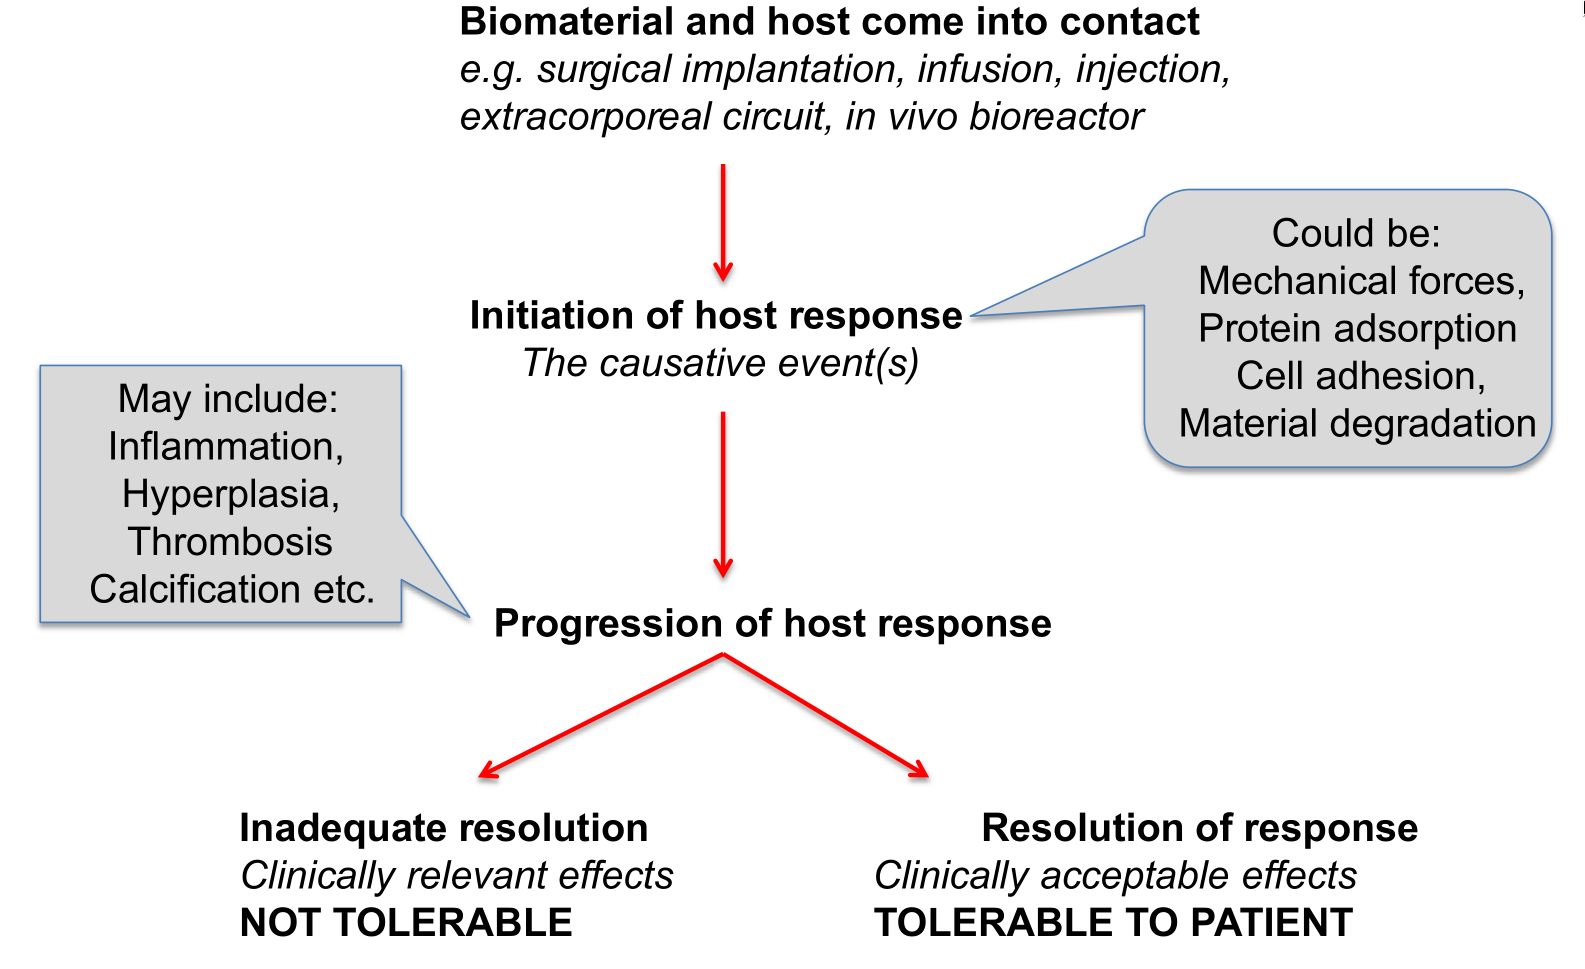
\includegraphics[width=0.7\textwidth]{biocomp_pathway.png}
		\caption{General biocompatibility pathway}
		\label{fig:biocomp_path}
	\end{figure}

	The simple generic pathway (figure \ref{fig:biocomp_path}) starts with the presentation of a clinical condition which leads to the decision to use a biomaterials-based therapy.
	The biomaterial may interact with cells in the determination of the appropriate host response.
	In most situations, the desired clinical outcome can only be achieved through a combination of effects on critical cells and the avoidance of effects on other cells.
	The part of the pathway between biomaterials and cells constitutes the generic biocompatibility pathway.
	The biomaterial will influence the events through mechanical or molecular signalling processes.

		\subsubsection{Cells}

		\begin{figure}[ht]
			\centering
			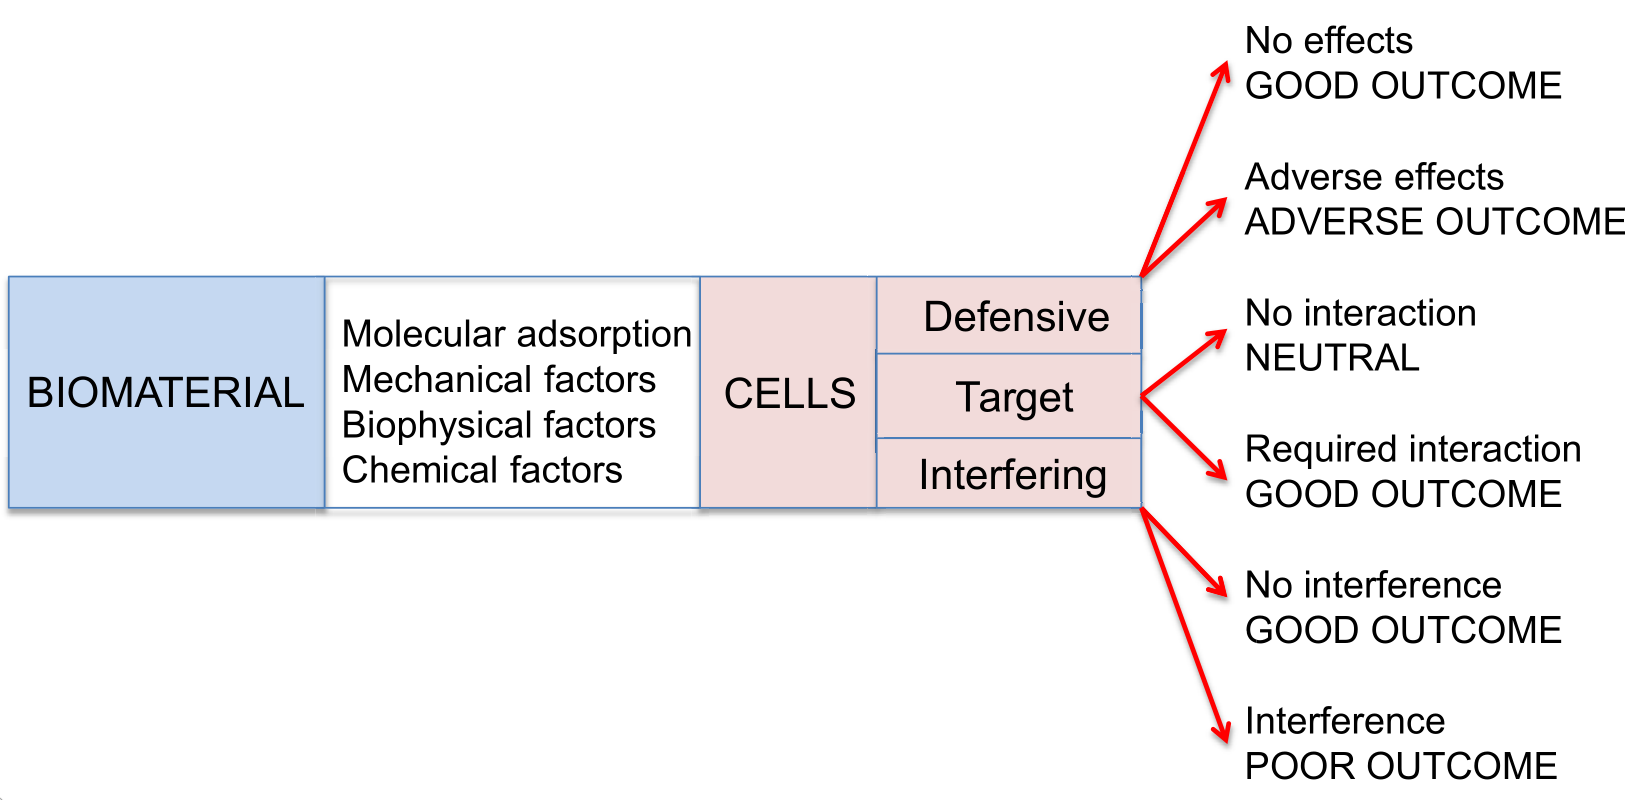
\includegraphics[width=0.8\textwidth]{biocomp_cells.png}
			\caption{Cells involved in a general biocompatibility pathway}
			\label{fig:biocomp_cells}
		\end{figure}

		Cells on this framework (figure \ref{fig:biocomp_cells}) can be:

		\begin{multicols}{2}
			\begin{itemize}
				\item Target cells: cells at which the therapy is aimed.
				\item Defensive cells: cells of innate and adaptive immunity, whose job is to repel and remove injurious external agents.
				\item Interfering cells: cells that interfere with the response that the biomaterial is seeking.
			\end{itemize}
		\end{multicols}

		The biocompatibility pathway will be determined by the events in these groups.
		The key to an appropriate host response is the dominance of the desirable effects over undesirable effects on the target cells, coupled with the avoidance of unacceptable responses via the defensive and interfering cells.
		The effects of chemical and mechanical events mediated by the biomaterial on cells are described on figure \ref{fig:biocomp_chem}


		\begin{figure}[ht]
			\centering
			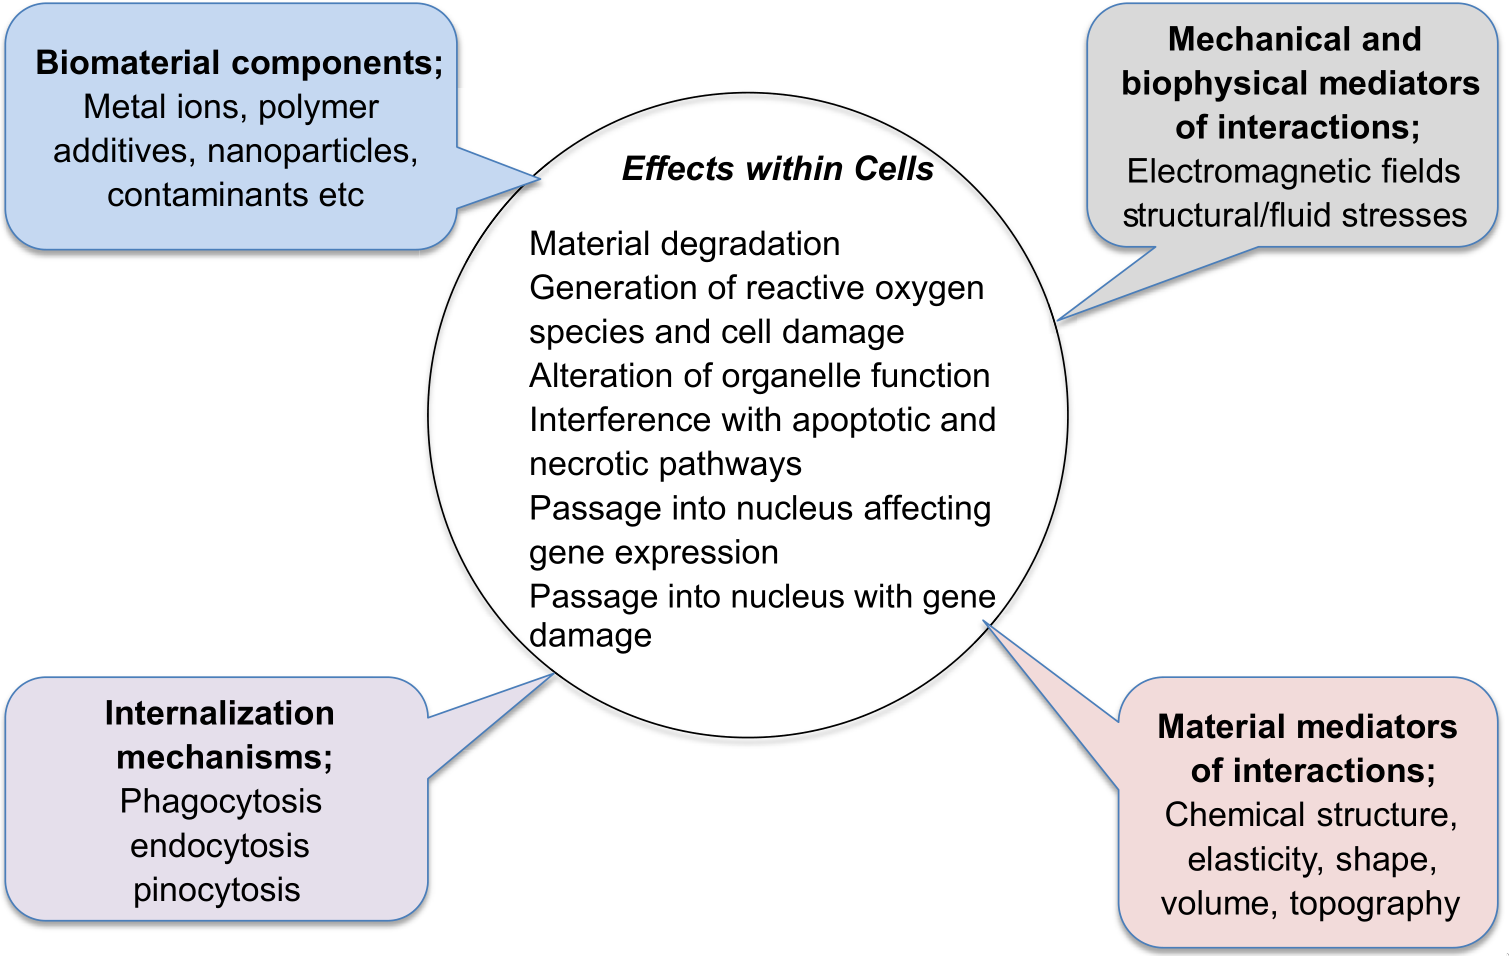
\includegraphics[width=0.8\textwidth]{biocomp_chem.png}
			\caption{Effects of biomaterial-mediated events on cells}
			\label{fig:biocomp_chem}
		\end{figure}

\section{The complexity of the biocompatible system}

\begin{figure}[ht]
	\centering
	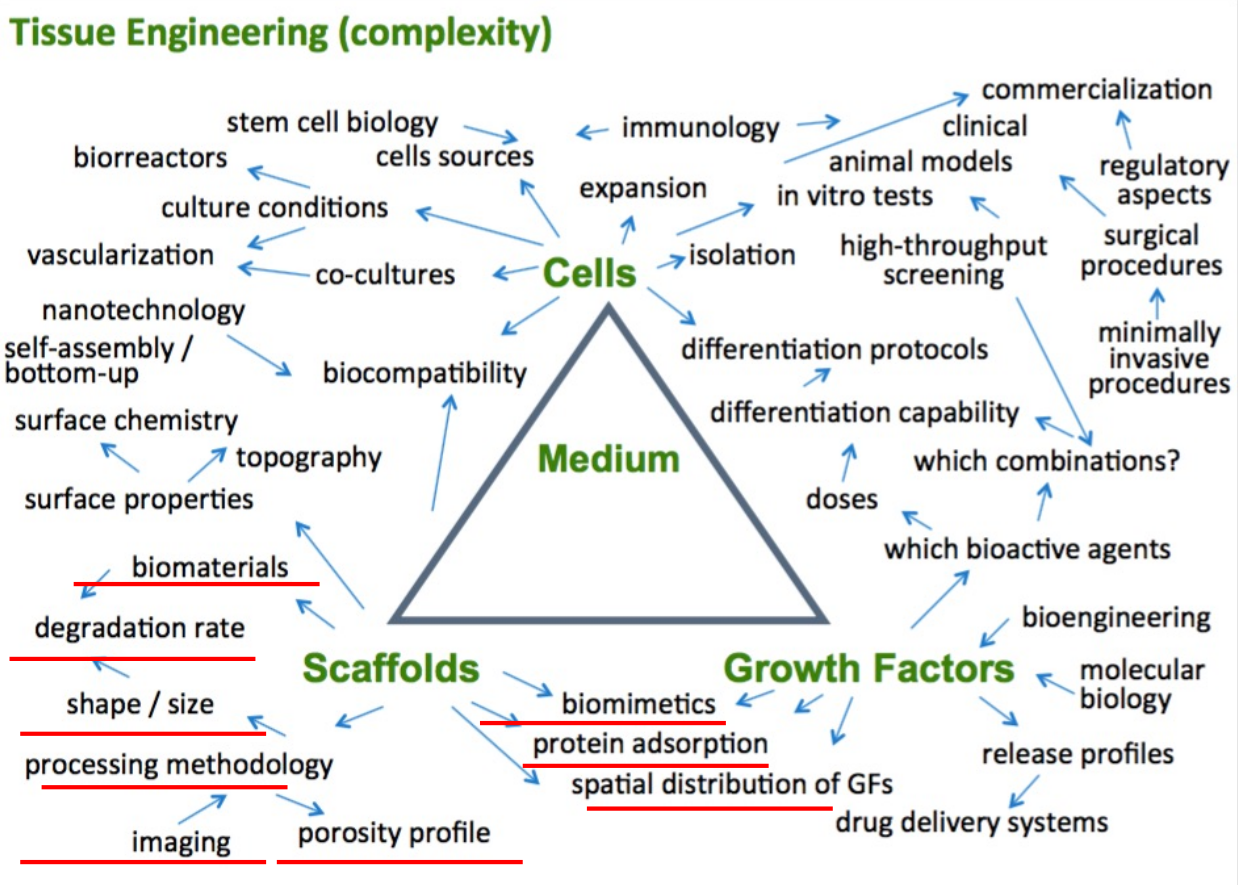
\includegraphics[width=0.7\textwidth]{piramide_completa.png}
	\caption{Tissue engineering can be represented by considering three actors\label{fig:complete_pyramid}}
\end{figure}

As it can be seen in figure \ref{fig:complete_pyramid}, only three actors are present in the tissue engineering paradigma, but each one has many ramification and possibilities.
\\
To design a biocompatible scaffold there is a need to take into account:

\begin{multicols}{2}
	\begin{itemize}
		\item Determination of native tissue or organ context.
		\item In vivo testing with bioreactors that provide a dynamic environment and mechanical stimuli by perfusion.
		\item Passage from in vitro to in vivo testing by selecting an appropriate animal model.
		\item Definition of the surgical model and finally we move to clinical trials.
	\end{itemize}
\end{multicols}

	\subsection{ECM molecules production: effect of the mechanical stimuli on a cartilage scaffold}

	\begin{figure}[ht]
		\centering
		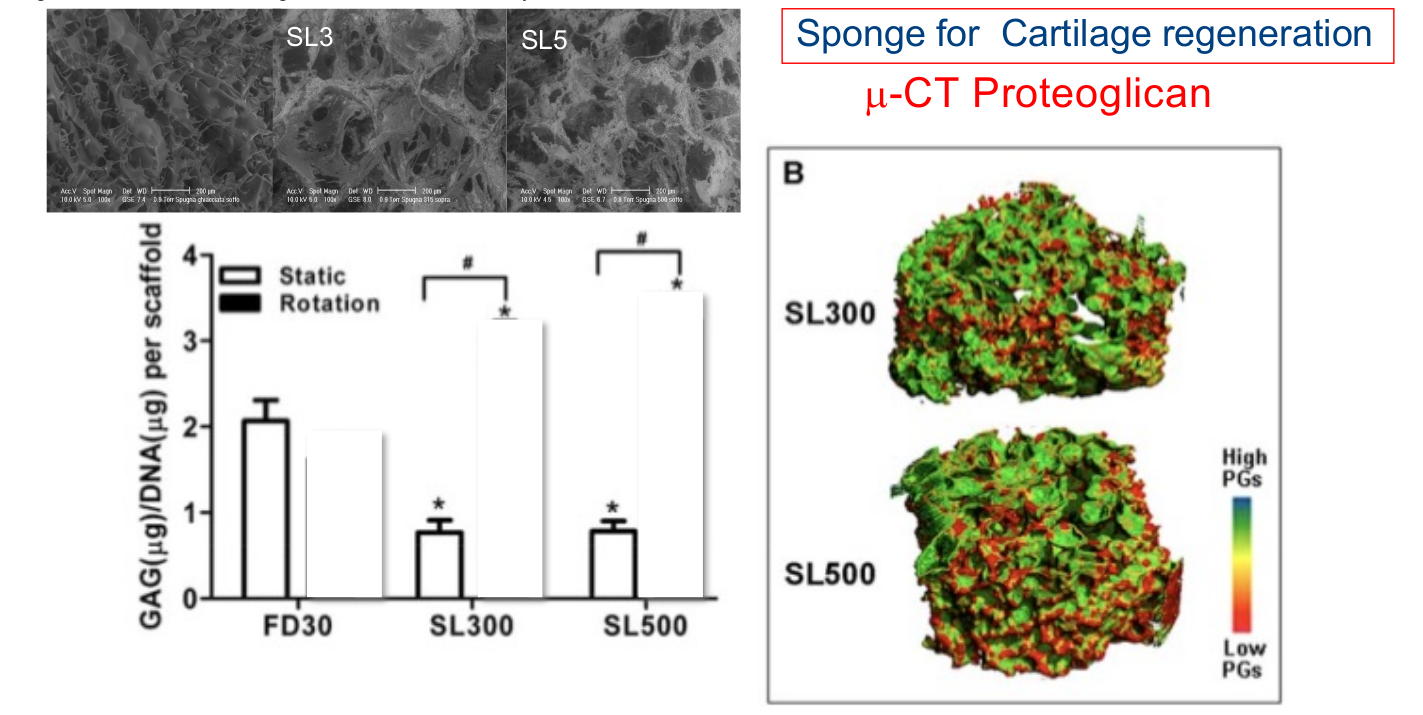
\includegraphics[width=0.5\textwidth]{sponge_cart.png}
		\caption{Cartilage sponges' quality assessment}
		\label{fig:sponge_c}
	\end{figure}

	Different sponge-like scaffolds were produced with different properties (like porosity) for cartilage regeneration.
	The quality of GAGs (glycosamminoglycans) into the ECM of cartilage was assessed.
	In addition, microCT - a 3D imaging technique - was used to see the level of infiltration of GAGs into the sponges.
	It can be seen in image \ref{fig:sponge_c} how SL500 had a lot of green, representing GAGs, but only on the outside of the sponge.
	When the sponges underwent a mechanical stress similar to the biological situation, the infiltration was also present on the inside.
	So, by changing from a static to a perfusion environment, the behaviour of molecules and sponges changed drastically.
	In particular, during perfusion integrins were upregulated.
	These molecules are transmembrane proteins responsible for cell to cell and cell to extracellular matrix communication; they are able to impart an instructive behaviour to cells, which are extremely sensible to it.
